We implemented the proposed approach to open-world mission specification in LTLMoP (the Linear Temporal Logic Mission Planning toolkit; see Section \ref{preliminariesB}). We augmented Structured English, one of LTLMoP's available specification languages, with \emph{open-world abstractions} (groups, quantifiers, and correspondences), the \emph{add to group} operator, and a \emph{resynthesis} action.

\begin{myExample}\label{Ex:mailbot3} We revisit the mailbot scenario from Examples \ref{Ex:mailbot1} and \ref{Ex:mailbot2}, and present the full mission specification, $\mathcal{M}_0$. The robot's workspace is depicted in Fig. \ref{Fig:map}.
\end{myExample}

Initially, the robot has no information about specific letters or their recipients. Therefore, it patrols the regions in \texttt{PatrolRooms}. If it senses a new letter, it will add a proposition to the group \texttt{Letters}. In simulation, LTLMoP prompts the user for the name of the proposition, e.g. \texttt{letter1}. Additionally, the \emph{add to} operator has to add a proposition to the group \texttt{Offices}, in order to maintain the correspondence. LTLMoP prompts the user a second time, and he inputs one of the region names, \texttt{r1}--\texttt{r6}. The two user prompts simulate the process of scanning the letter for the recipient's name and address, in order to name and ground the new propositions (see Assumption \ref{Ass:grounding}).

\begin{algorithm}
	\textbf{Mission specification:} Autonomous Mailbot
	
	\vspace{-7 pt}
	\hrulefill\\
	{\small
	
	\textbf{Group declarations:}\\
	\texttt{Group Letters is empty} \\
%	\texttt{Group LetterSlots is empty} \\
%	\texttt{Group Delivery is empty} \\
	\texttt{Group Offices is empty} \\
	\texttt{Group PatrolRooms is mailRoom, hallW, hallN}\\ % FIXME: I don't like 'hall_x"s
	
	\textbf{Correspondence definitions:} (immutable)\\ %FIXME: Add more for add_to to work?
%	\texttt{Letters correspond to LetterSlots, Delivery, Offices}\\ %FIXME: This isn't implemented
%	\texttt{LetterSlots correspond to Letters}\\
%	\texttt{LetterSlots correspond to Delivery}\\
%	\texttt{Delivery correspond to LetterSlots}\\
%	\texttt{Delivery correspond to Offices}\\
	\texttt{Letters correspond to Offices}\\
	
%	\hrulefill\\
	% TODO: We can't have initial conditions when we are re-synthesizing, right?
%	\textbf{Initial conditions} (optional)\\
%	\texttt{Robot starts in mailRoom with false}\\
%	\texttt{Environment starts with false}\\
	
	\textbf{Mission tasks:} (immutable)\\
	\texttt{If you are sensing any Letters then go to the corresponding Office}\\
	\texttt{If you are not sensing any Letters then visit each PatrolRoom}\\
%	\texttt{Each LetterSlot is set on the corresponding Letter and pickUp and reset on the corresponding Delivery}\\
	
%	\texttt{Do pickUp if and only if you are sensing any Letters}\\
%	\texttt{If you are activating pickUp then stay there}\\
	
%	\texttt{Do each Delivery if and only if you are in the corresponding Office and you are activating the corresponding LetterSlot}\\
	
%	\texttt{Infinitely often not each LetterSlot}\\
%	\texttt{If you are not activating any LetterSlots then visit each PatrolRooms}\\
	
	\textbf{Open--World settings:} (immutable)\\
	\texttt{If you are sensing newLetter then add to group Letters and resynthesize}\\
	\texttt{If you are sensing newLetter then stay there}\\
		
	\textbf{Environment fairness assumption:} (immutable)\\
%	\texttt{Infinitely often not any Letters}\\
	\texttt{Infinitely often not newLetter}\\
	}
	\vspace{-10 pt}
\end{algorithm}

\begin{figure}[h]
	\centering
	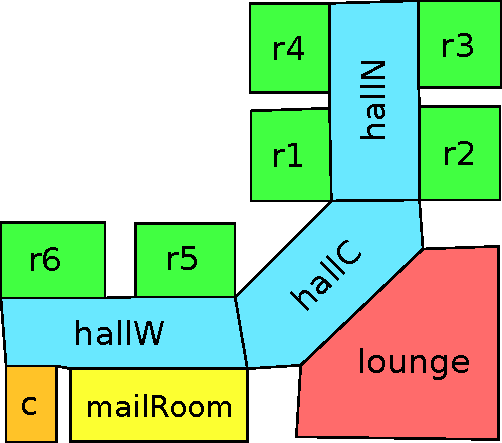
\includegraphics[width=0.80\columnwidth, clip]{./img/mailbot_map.pdf}
	\caption{Map of workspace for mailbot scenario.  Regions \texttt{r1}--\texttt{r6} are the offices of potential letter recipients.} 
	\label{Fig:map}
\end{figure}

After the specification is rewritten, the LTL formula $\varphi [k]$ changes to $\varphi [k+1]$, according to Eqs. \eqref{Eq:newSpecA} and \eqref{Eq:newSpecB}. The change involved adding a new mission goal: the delivery of \texttt{letter1} to the corresponding office \texttt{r1}. Specifically, compared to $\varphi_g^s [k]$, $\varphi_g^s [k+1]$ contains the additional liveness requirement:
\begin{equation*}
	\G\F\left( \texttt{letter1} \Rightarrow \texttt{r1} \right)
\end{equation*}

After resynthesis, the robot can now sense letters in two ways. First, it could detect a letter addressed to the same recipient as \texttt{letter1}. In this case, \texttt{letter1} will become \texttt{True}, and the robot will deliver the letter to \texttt{r1}. Second, it could detect a letter addressed to a new recipient. In that case, the sensor \texttt{newLetter} will become \texttt{True}, and the \emph{add to group} operator will once again cause new propositions to be added to \texttt{Letters} and \texttt{Offices}.

% END
%
%\begin{myExample}\label{Ex:restaurant} Robotic Waiter \\
%	Overview of task \ldots
%\end{myExample}
%
%\begin{algorithm}
%	\textbf{Mission specification:} Robotic Waiter\\
%	{\small
%	\texttt{Group Customers is empty}\\
%	\texttt{Group Orders is empty}\\
%	\texttt{Group ... is empty}\\
%	\texttt{Group ... is empty}\\
%	
%	\texttt{Orders correspond to Customers}\\
%	\texttt{... correspond to...}\\
%	
%	\texttt{if you are activating any Orders then go to kitchen and do corresponding FoodPickUp and go to corresponding Customer and do corresponding ServeFood}\\
%	\texttt{...}\\
%	
%	\texttt{...}\\
%	}
%	
%	\textbf{Open World Settings:}\\
%	{\small
%	\texttt{if you are sensing newOrder then add to Orders}\\ % TODO: ... and add to corr. groups?
%	\texttt{...} 
%	}
%\end{algorithm}
%
%\begin{myExample}\label{Ex:planetxplore} Autonomous Planetary Exploration\\
%	Consider now the more futuristic scenario of autonomous planetary exploration using rovers. In order to lessen the dependency of the rover from the engineers on Earth, the rover will be given a mission specification that it should carry out autonomously. However, the need to redefine the mission will arise as the rover discovers interesting elements of its environment, such as new types of rock and regions interest. In these cases, the engineers and scientists on Earth should be able to extend the rover's mission specification without sacrificing correctness or rewriting the specification from scratch.
%	
%	Specifics: exploration, new stuff sensor, new requests.
%\end{myExample}
%
%\begin{algorithm}
%	\textbf{Mission specification:} Autonomous Planetary Exploration\\
%	{\small
%	\texttt{Group InterestingRegions is empty}\\
%	\texttt{Group PendingRequests is empty}\\
%	\texttt{Group Sites is empty}\\
%	\texttt{Group Actions is empty}\\
%	
%	\texttt{Sites correspond to Requests}\\
%	\texttt{Actions correspond to Requests}\\
%	
%	\texttt{Recharging is set on BatteryLow and reset on BatteryFull}\\
%	\texttt{if you are activating Recharging then stay there}\\
%	\texttt{infinitely often BatteryFull}\\
%	
%	\texttt{visit each InterestingRegion and do Panorama}\\
%	\texttt{if you are activating any PendingRequests then go to the corresponding Site and do the corresponding Action}\\
%	\texttt{each PendingRequest is toggled on the corresponding Site and the corresponding Action}\\
%	}
%	
%	\textbf{Exploration Settings:}\\
%	{\small
%	\texttt{do exploreMODE if and only if you are not activating Recharging}\\
%	\texttt{if you are sensing newInterestingRegion then add to InterestingRegions}\\
%	\texttt{...} 
%	}
%\end{algorithm}
%
%\begin{figure}[h]
%	\centering
%	\includegraphics[width=0.7\columnwidth, clip]{./img/planetXplore_regions.pdf}
%	\caption{Workspace for the autonomous planetary exploration scenario (to be updated and broken down to intermediate exploration steps).}
%	% TODO: Update this map. Regions should be around the land site! No mountain next to it either.
%	% Instead of the final map, show intermediate steps as the workspace is expanded.
%	\label{Fig:planetxplore}
%\end{figure}